\documentclass[11pt]{article}

\usepackage{amsmath}
\usepackage{amssymb}
\usepackage{booktabs}
\usepackage{enumitem}
\usepackage[T1]{fontenc}
\usepackage[margin=1in]{geometry}
\usepackage{graphicx}
\usepackage[utf8]{inputenc}
\usepackage{libertine}
\usepackage[libertine]{newtxmath}
\usepackage{pgfplots}

\title{MATH 128 End-of-Term Assignment 2}
\author{Brandon Tsang}
\date{April 5, 2020}

\usepgfplotslibrary{polar}
\pgfplotsset{
    compat=1.16,
    every axis/.append style={
        scale only axis,
        y label style={rotate=-90},
        minor tick num=1,
        grid=both,
        minor grid style={black!10},
    }
}

\begin{document}
    \maketitle
    \begin{enumerate}[label=\textbf{\arabic*.}]
        \item{
            \textbf{\boldmath Consider the function \(f(x,y)=\sqrt{x^2+y^2}\).}
            \begin{enumerate}[label=\textbf{(\alph*)}]
                \item{
                    \textbf{\boldmath State the domain and range of \(f\).}
                    \par
                    The expression under the radical must be greater than or equal to zero (i.e., \(x^2+y^2\ge0\)). However, \(x^2\) and \(y^2\) are always positive or zero, so the domain is \(\{x,y\in\mathbb{R}\}\).
                    \par
                    The range is \(\{z\in\mathbb{R}\mid z\ge0\}\) since a square root is always positive or zero.
                }
                \item{
                    \label{part:1b}
                    \textbf{\boldmath Sketch a contour plot of \(f(x,y)\) illustrating the level curves defined by \(f(x,y)=k\) for \(k=0,1,2,3\).}
                    \def\axiswidth{2in}
                    \def\axisheight{2in}
                    \begin{center}
                        \begin{tikzpicture}
                            \begin{axis}[
                                width=\axiswidth,
                                height=\axisheight,
                                title={Contour plot for \(k=0\)},
                                xlabel={\(x\)},
                                ylabel={\(y\)},
                                xmin=-4, xmax=4,
                                ymin=-4, ymax=4
                            ]
                            \end{axis}
                        \end{tikzpicture}
                        \hspace{14pt}
                        \begin{tikzpicture}
                            \begin{axis}[
                                width=\axiswidth,
                                height=\axisheight,
                                title={Contour plot for \(k=1\)},
                                xlabel={\(x\)},
                                ylabel={\(y\)},
                                xmin=-4, xmax=4,
                                ymin=-4, ymax=4
                            ]
                                \node at (0,0) {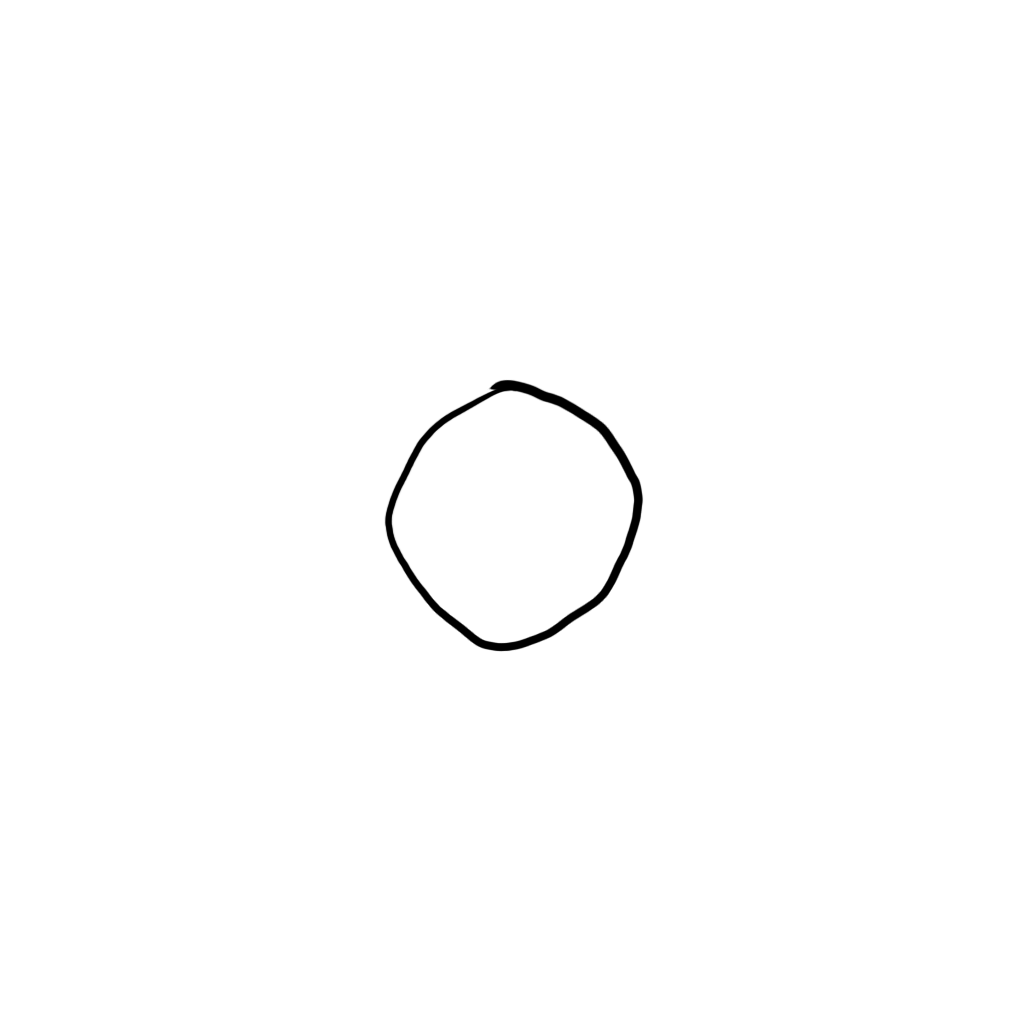
\includegraphics[width=\axiswidth]{k1.png}};
                            \end{axis}
                        \end{tikzpicture}
                    \end{center}
                    \begin{center}
                        \begin{tikzpicture}
                            \begin{axis}[
                                width=\axiswidth,
                                height=\axisheight,
                                title={Contour plot for \(k=2\)},
                                xlabel={\(x\)},
                                ylabel={\(y\)},
                                xmin=-4, xmax=4,
                                ymin=-4, ymax=4
                            ]
                                \node at (0,0) {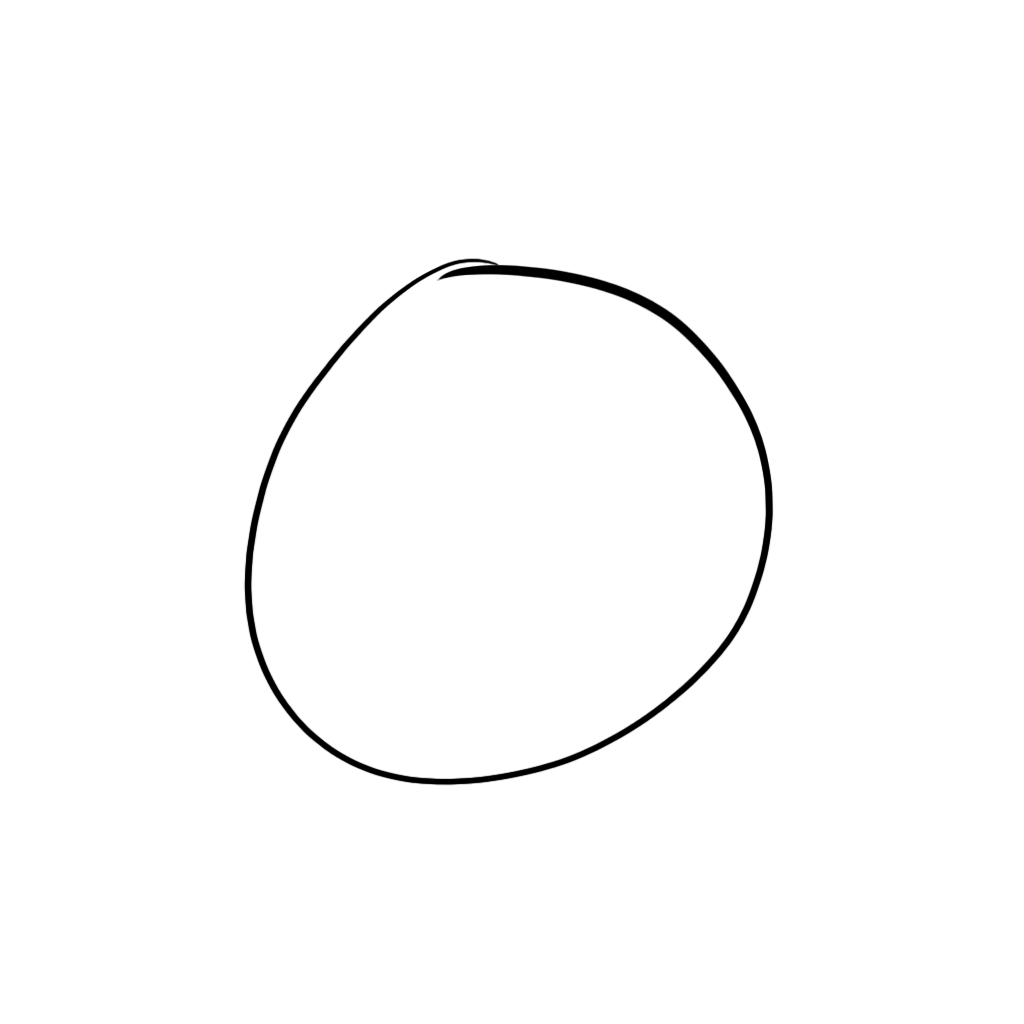
\includegraphics[width=\axiswidth]{k2.png}};
                            \end{axis}
                        \end{tikzpicture}
                        \hspace{14pt}
                        \begin{tikzpicture}
                            \begin{axis}[
                                width=\axiswidth,
                                height=\axisheight,
                                title={Contour plot for \(k=3\)},
                                xlabel={\(x\)},
                                ylabel={\(y\)},
                                xmin=-4, xmax=4,
                                ymin=-4, ymax=4
                            ]
                                \node at (0,0) {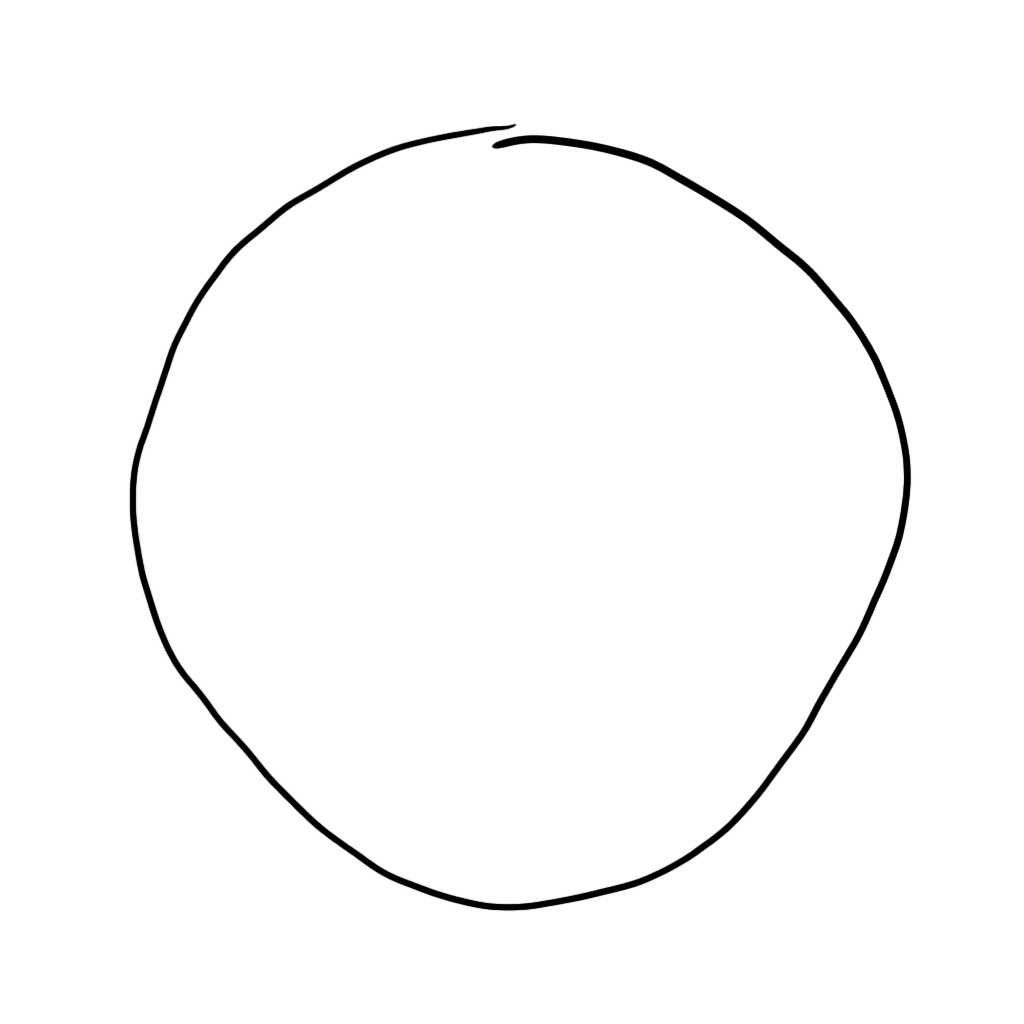
\includegraphics[width=\axiswidth]{k3.png}};
                            \end{axis}
                        \end{tikzpicture}
                    \end{center}
                }
                \item{
                    \label{part:1c}
                    \textbf{\boldmath Consider the surface \(z=f(x,y)\). Determine equations for the cross-sections \(z=f(0,y)\) and \(z=f(x,0)\) (i.e., the curves of intersection between the surface and the \(yz\) and \(xz\) planes, respectively).}
                    \par
                    For \(z=f(0,y)\):
                    \begin{align*}
                        z&=\sqrt{0^2+y^2} \\
                        &=\sqrt{y^2} \\
                        &=|y|
                    \end{align*}
                    And for \(z=f(x,0)\):
                    \begin{align*}
                        z&=\sqrt{x^2+0^2} \\
                        &=\sqrt{x^2} \\
                        &=|x|
                    \end{align*}
                }
                \item{
                    \textbf{\boldmath Sketch (by hand) a graph of the surface \(z=f(x,y)\). Make the graph large enough so as to be able to draw and label the curves you found in part \ref{part:1b} and the cross-sections you found in part \ref{part:1c} on the surface.}
                    \begin{center}
                        \begin{tikzpicture}
                            \begin{axis}[
                                width=6in,
                                height=5in,
                                axis lines=middle,
                                axis line style={shorten >=-10pt},
                                xmin=-4, xmax=4,
                                ymin=-4, ymax=4,
                                zmin=0, zmax=5,
                                xlabel={\(x\)},
                                ylabel={\(y\)},
                                y label style={at=(yticklabel* cs:1), right=8pt},
                                zlabel={\(z\)}
                            ]
                                \node at (0.1,0,1.6) {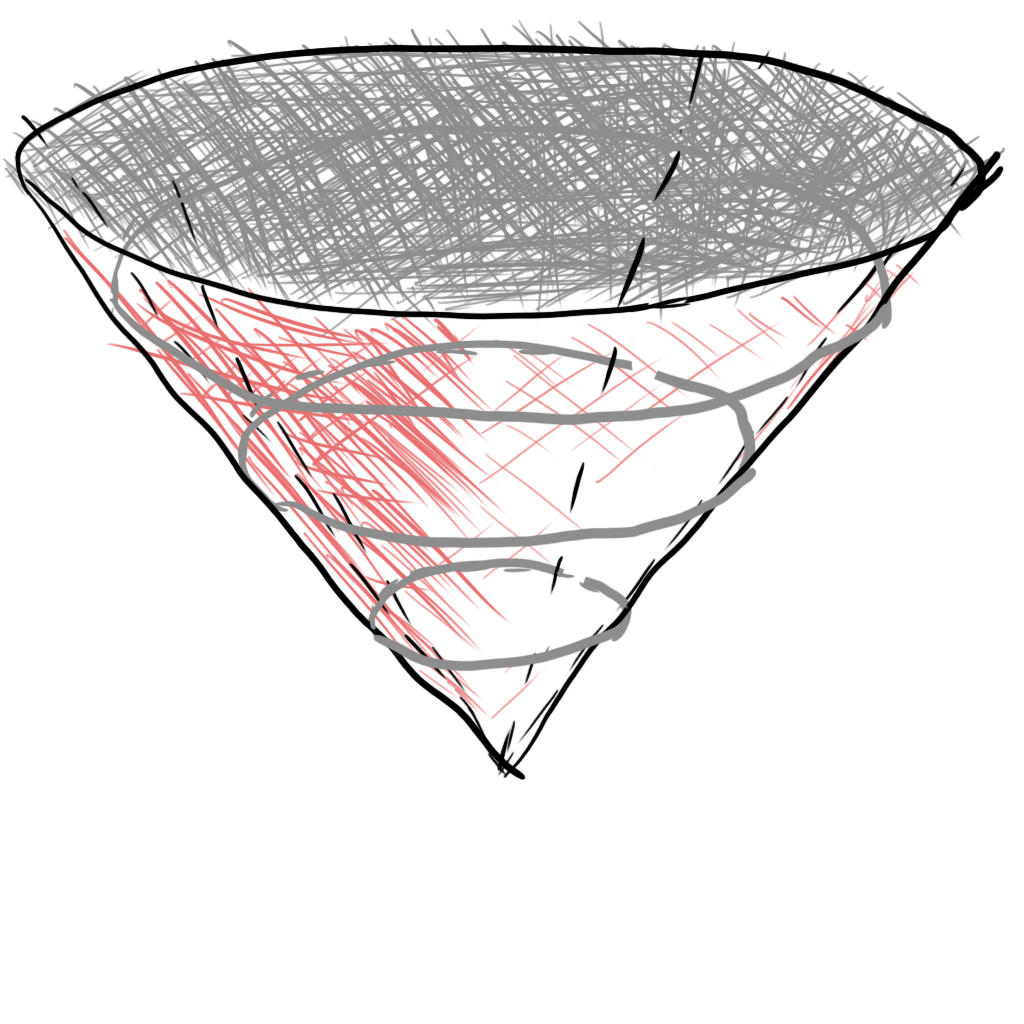
\includegraphics[width=4.5in, height=3.5in]{1d.png}};
                                \node at (-0.8,-0.6,1) [anchor=north east] {\(k=1\)};
                                \node at (-1.6,-1.2,2) [anchor=north east] {\(k=2\)};
                                \node at (-2.7,-1.4,3) [anchor=north east] {\(k=3\)};
                                \node at (0.2,3.3,3.3) [anchor=south west] {\(z=f(0,y)\)};
                                \node at (-3.9,0,3.3) [anchor=south east] {\(z=f(x,0)\)};
                            \end{axis}
                        \end{tikzpicture}
                    \end{center}
                }
            \end{enumerate}
        }
        \pagebreak
        \item{
            \begin{enumerate}[label=\textbf{(\alph*)}]
                \item{
                    \textbf{\boldmath Convert \((r,\theta)=\left(2,\frac{\pi}{6}(N_7+1)\right)\) to Cartesian coordinates where \(N_7\) is the seventh digit of your student number.}
                    \par
                    My student number is 20845794, so \(N_7=9\). \(\frac{\pi}{6}(N_7+1)\) then becomes \(\frac{5\pi}{3}\). Finding \(x\):
                    \begin{align*}
                        x&=r\cos\theta \\
                        &=2\cos\frac{5\pi}{3} \\
                        &=2\cdot\frac{1}{2} \\
                        &=1
                    \end{align*}
                    Then, finding \(y\):
                    \begin{align*}
                        y&=r\sin\theta \\
                        &=2\sin\frac{5\pi}{3} \\
                        &=2\cdot-\frac{\sqrt3}{2} \\
                        &=-\sqrt 3
                    \end{align*}
                    So \(\left(2,\frac{\pi}{6}(N_7+1)\right)\) in Cartesian coordinates is \(\left(1,-\sqrt3\right)\).
                }
                \item{
                    \textbf{\boldmath Convert \((x,y)=\left(-\sqrt3(N_8+1),N_8+1\right)\) to polar coordinates where \(N_8\) is the eighth digit of your student number.}
                    \par
                    \(N_8=4\), so \(x=-\sqrt3(N_8+1)\) becomes \(x=5\sqrt3\) and \(y=N_8+1\) becomes \(y=5\). Finding \(r\):
                    \begin{align*}
                        r&=\sqrt{x^2+y^2} \\
                        &=\sqrt{\left(5\sqrt3\right)^2+5^2} \\
                        &=\sqrt{75+25} \\
                        &=10
                    \end{align*}
                    Then, finding \(\theta\):
                    \begin{align*}
                        \theta&=\tan^{-1}\frac{y}{x} \\
                        &=\tan^{-1}\frac{5}{5\sqrt3} \\
                        &=\tan^{-1}\frac{1}{\sqrt3} \\
                        &=\frac{\pi}{6}
                    \end{align*}
                    So \(\left(-\sqrt3(N_8+1),N_8+1\right)\) in polar coordinates is \(\left(10,\frac{\pi}{6}\right)\).
                }
                \pagebreak
                \item{
                    \textbf{\boldmath In the \(xy\)-plane, sketch the curve defined by \(r(\theta)=2\) for \(0\le\theta\le2\pi\).}
                    \begin{center}
                        \begin{tikzpicture}
                            \begin{polaraxis}[
                                width=3in,
                                height=3in,
                                xticklabels={0,0,\(\frac{\pi}{6}\),\(\frac{\pi}{3}\),\(\frac{\pi}{2}\),\(\frac{2\pi}{3}\),\(\frac{5\pi}{6}\),\(\pi\),\(\frac{7\pi}{6}\),\(\frac{4\pi}{3}\),\(\frac{3\pi}{2}\),\(\frac{5\pi}{3}\),\(\frac{11\pi}{6}\)},
                                ymax=2.5
                            ]
                                \node at (0,0) {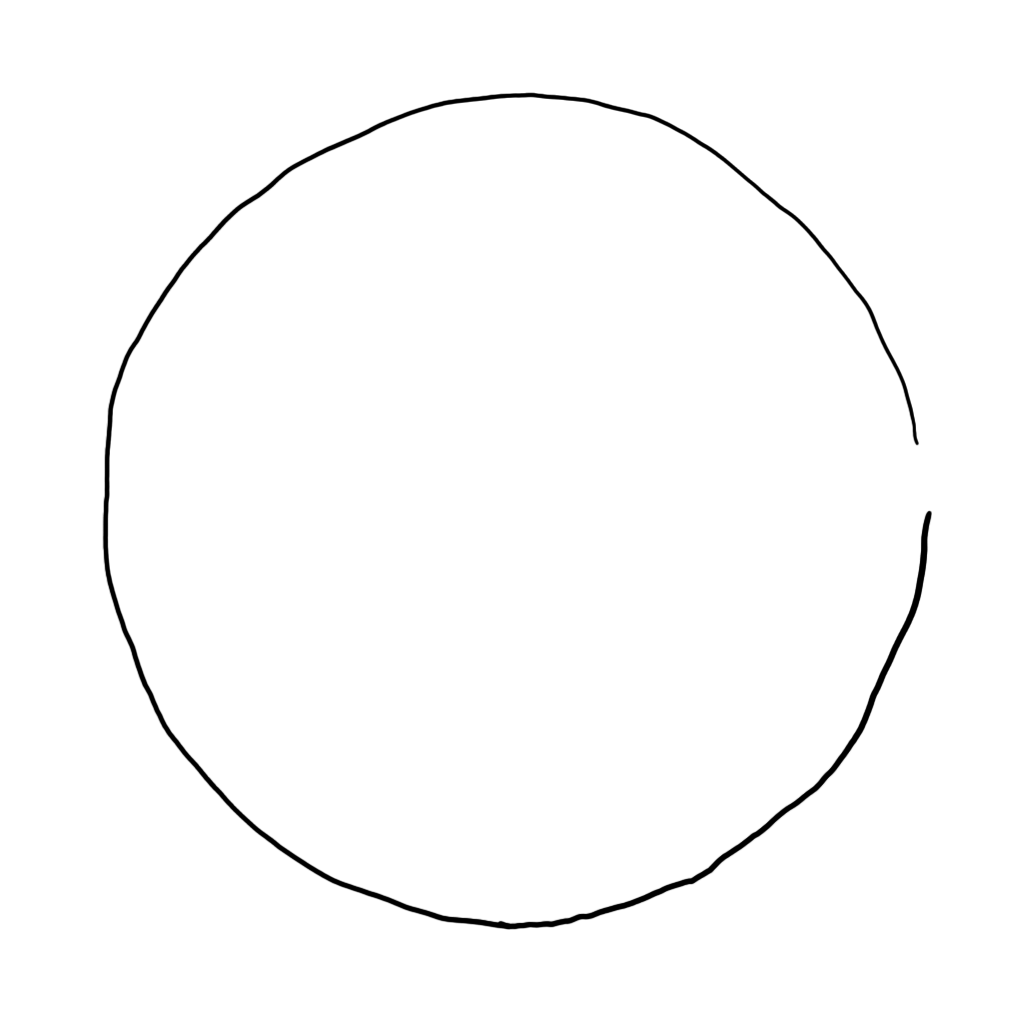
\includegraphics[width=3in]{2c.png}};
                            \end{polaraxis}
                        \end{tikzpicture}
                    \end{center}
                }
                \item{
                    \textbf{\boldmath In the \(xy\)-plane, sketch the curve defined by \(r(\theta)=2\cos\theta+2\sin\theta\) for \(0\le\theta\le\pi\).}
                    \begin{center}
                        \begin{tikzpicture}
                            \begin{polaraxis}[
                                width=3in,
                                height=3in,
                                xticklabels={0,0,\(\frac{\pi}{6}\),\(\frac{\pi}{3}\),\(\frac{\pi}{2}\),\(\frac{2\pi}{3}\),\(\frac{5\pi}{6}\),\(\pi\),\(\frac{7\pi}{6}\),\(\frac{4\pi}{3}\),\(\frac{3\pi}{2}\),\(\frac{5\pi}{3}\),\(\frac{11\pi}{6}\)},
                                ymax=3.2
                            ]
                                \node at (0,0) {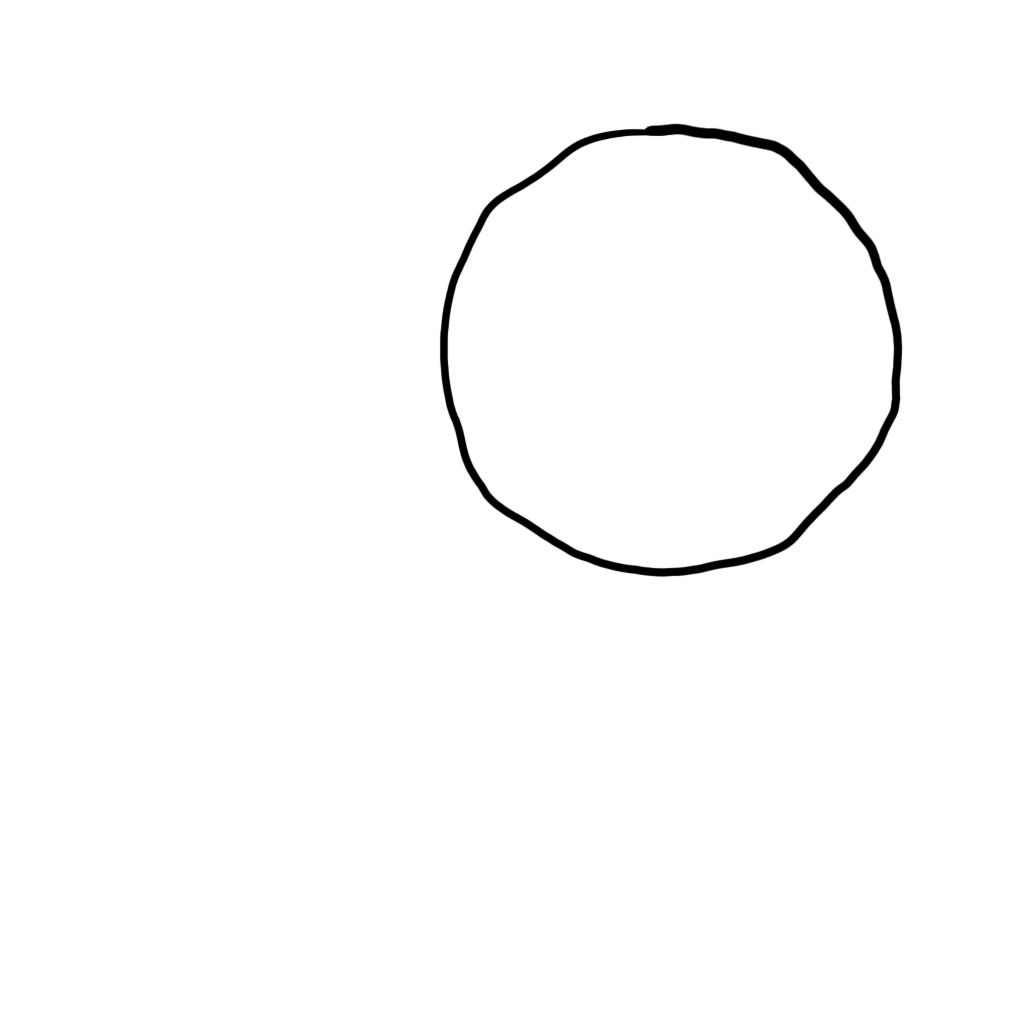
\includegraphics[width=3in]{2d.png}};
                            \end{polaraxis}
                        \end{tikzpicture}
                    \end{center}
                }
            \end{enumerate}
        }
        \pagebreak
        \item{
            \textbf{\boldmath Let \(f(x,y)=\sqrt{xy}\).}
            \begin{enumerate}[label=\textbf{(\alph*)}]
                \item{
                    \textbf{\boldmath Compute the first partial derivatives of \(f(x,y)\).}
                    \par
                    With respect to \(x\):
                    \begin{align*}
                        \frac{\partial f}{\partial x}&=\sqrt y\left(\frac{1}{2}x^{-\frac{1}{2}}\right) \\
                        &=\frac{\sqrt y}{2\sqrt x}
                    \end{align*}
                    And with respect to \(y\):
                    \begin{align*}
                        \frac{\partial f}{\partial y}&=\sqrt x\left(\frac{1}{2}y^{-\frac{1}{2}}\right) \\
                        &=\frac{\sqrt x}{2\sqrt y}
                    \end{align*}
                }
                \item{
                    \textbf{\boldmath Compute the second partial derivatives of \(f(x,y)\).}
                    \par
                    First, \(f_{xx}(x,y)\):
                    \begin{align*}
                        \frac{\partial^2f}{\partial x^2}&=\frac{\partial}{\partial x}\left(\frac{\sqrt y}{2\sqrt x}\right) \\
                        &=\frac{\sqrt y}{2}\left(-\frac{1}{2}x^{-\frac{3}{2}}\right) \\
                        &=-\frac{\sqrt y}{4x^{\frac{3}{2}}}
                    \end{align*}
                    Next, \(f_{yy}(x,y)\):
                    \begin{align*}
                        \frac{\partial^2f}{\partial y^2}&=\frac{\partial}{\partial y}\left(\frac{\sqrt x}{2\sqrt y}\right) \\
                        &=\frac{\sqrt x}{2}\left(-\frac{1}{2}y^{-\frac{3}{2}}\right) \\
                        &=-\frac{\sqrt x}{4y^{\frac{3}{2}}}
                    \end{align*}
                    Since \(f_{xy}(x,y)=f_{yx}(x,y)\), I will only compute \(f_{xy}(x,y)\).
                    \begin{align*}
                        f_{xy}(x,y)&=\frac{\partial}{\partial y}\left(\frac{\sqrt y}{2\sqrt x}\right) \\
                        &=\frac{1}{2\sqrt x}\left(\frac{1}{2}y^{-\frac{1}{2}}\right) \\
                        &=\frac{1}{4\sqrt{xy}}
                    \end{align*}
                }
                \pagebreak
                \item{
                    \label{part:3c}
                    \textbf{\boldmath Find an equation for the plane tangent to the surface \(z=f(x,y)\) when \((x,y)=(1,1)\).}
                    \par
                    The equation for a plane tangent to the surface of a function \(f(x,y)\) at \(x=x_0\) and \(y=y_0\) is
                    \begin{equation*}
                        z=f(x_0,y_0)+f_x(x_0,y_0)\cdot(x-x_0)+f_y(x_0,y_0)\cdot(y-y_0).
                    \end{equation*}
                    Finding the coefficients:
                    \begin{align*}
                        f(1,1)&=\sqrt{1\cdot1} \\
                        &=1
                    \end{align*}
                    \begin{align*}
                        f_x(1,1)&=\frac{\sqrt1}{2\sqrt1} \\
                        &=\frac{1}{2}
                    \end{align*}
                    \begin{align*}
                        f_y(1,1)&=\frac{\sqrt1}{2\sqrt1} \\
                        &=\frac{1}{2}
                    \end{align*}
                    Then, putting it all together:
                    \begin{align*}
                        z&=1+\frac{1}{2}(x-1)+\frac{1}{2}(y-1) \\
                        &=1+\frac{x}{2}-\frac{1}{2}+\frac{y}{2}-\frac{1}{2} \\
                        &=\frac{x+y}{2}
                    \end{align*}
                }
                \item{
                    \textbf{\boldmath Determine the linearization of \(f(x,y)\) at \((x,y)=(1,1)\) and use it to approximate \(f(1.1,0.8)\).}
                    \par
                    The linearization of \(f(x,y)\) is the equation of the plane from part \ref{part:3c}.
                    \begin{align*}
                        f(x,y)&\approx\frac{x+y}{2} \\
                        f(1.1,0.8)&\approx\frac{1.1+0.8}{2} \\
                        &\approx0.95
                    \end{align*}
                }
            \end{enumerate}
        }
        \pagebreak
        \item{
            \textbf{\boldmath The wave equation is a partial differential equation which, for waves propagating in one spatial dimension, is given by \[f_{tt}(x,t)=a^2f_{xx}(x,t)\] where \(x\) is position, \(t\) is time, and \(a\) is a constant. Determine whether each of the following functions is a solution to the wave equation:}
            \begin{enumerate}[label=\textbf{(\alph*)}]
                \item{
                    \textbf{\boldmath \(f(x,t)=\sin(x)\cos(at)\)}
                    \par
                    Taking two partial derivatives with respect to \(t\):
                    \begin{align*}
                        \frac{\partial f}{\partial t}&=\sin(x)\cdot-a\sin(at) \\
                        \frac{\partial^2f}{\partial t^2}&=-a\sin(x)\cdot a\cos(at) \\
                        &=-a^2\sin(x)\cos(at)
                    \end{align*}
                    Then with respect to \(x\):
                    \begin{align*}
                        \frac{\partial f}{\partial x}&=\cos(at)\cos(x) \\
                        \frac{\partial^2f}{\partial x^2}&=\cos(at)\cdot-\sin(x) \\
                        &=-\sin(x)\cos(at)
                    \end{align*}
                    Then,
                    \begin{align*}
                        f_{tt}(x,t)&\stackrel{?}{=}a^2f_{xx}(x,t) \\
                        -a^2\sin(x)\cos(at)&\stackrel{?}{=}a^2(-\sin(x)\cos(at)) \\
                        -a^2\sin(x)\cos(at)&=-a^2\sin(x)\cos(at)
                    \end{align*}
                    so \(f(x,t)=\sin(x)\cos(at)\) is a solution.
                }
                \item{
                    \textbf{\boldmath \(f(x,t)=e^{-at}\sin(x)\)}
                    \par
                    Taking two partial derivatives with respect to \(t\):
                    \begin{align*}
                        \frac{\partial f}{\partial t}&=\sin(x)\cdot-ae^{-at} \\
                        \frac{\partial^2f}{\partial t^2}&=-a\sin(x)\cdot-ae^{-at} \\
                        &=a^2e^{-at}\sin(x)
                    \end{align*}
                    Then with respect to \(x\):
                    \begin{align*}
                        \frac{\partial f}{\partial x}&=e^{-at}\cos(x) \\
                        \frac{\partial^2f}{\partial x}&=e^{-at}\cdot-\sin(x) \\
                        &=-e^{-at}\sin(x)
                    \end{align*}
                    Then,
                    \begin{align*}
                        f_{tt}(x,t)&\stackrel{?}{=}a^2f_{xx}(x,t) \\
                        a^2e^{-at}\sin(x)&\stackrel{?}{=}a^2(-e^{-at}\sin(x)) \\
                        a^2e^{-at}\sin(x)&\neq-a^2e^{-at}\sin(x)
                    \end{align*}
                    so \(f(x,t)=e^{-at}\sin(x)\) is not a solution.
                }
                \item{
                    \textbf{\boldmath \(f(x,t)=(x-at)^4\)}
                    \par
                    Taking two partial derivatives with respect to \(t\):
                    \begin{align*}
                        \frac{\partial f}{\partial t}&=4(x-at)^3\cdot-a \\
                        \frac{\partial^2f}{\partial t^2}&=-4a\cdot3(x-at)^2\cdot-a \\
                        &=12a^2(x-at)^2
                    \end{align*}
                    Then with respect to \(x\):
                    \begin{align*}
                        \frac{\partial f}{\partial x}&=4(x-at)^3 \\
                        \frac{\partial^2f}{\partial x}&=12(x-at)^2
                    \end{align*}
                    Then,
                    \begin{align*}
                        f_{tt}(x,t)&\stackrel{?}{=}a^2f_{xx}(x,t) \\
                        12a^2(x-at)^2&\stackrel{?}{=}a^2\cdot12(x-at)^2 \\
                        12a^2(x-at)^2&=12a^2(x-at)^2 \\
                    \end{align*}
                    so \(f(x,t)=(x-at)^4\) is a solution.
                }
            \end{enumerate}
        }
        \item{
            \textbf{Evaluate the following iterated integrals:}
            \begin{enumerate}[label=\textbf{(\alph*)}]
                \item{
                    \textbf{\boldmath \(\int_{x=0}^2\int_{y=0}^2x^2y^2\,dy\,dx\)}
                    \begin{align*}
                        \int_{x=0}^2\int_{y=0}^2x^2y^2\,dy\,dx&=\int_0^2x^2\left[\frac{1}{3}y^3\right]_0^2\,dx \\
                        &=\frac{8}{3}\int_0^2x^2\,dx \\
                        &=\frac{8}{3}\left[\frac{1}{3}x^3\right]_0^2 \\
                        &=\frac{8}{3}\left(\frac{8}{3}\right) \\
                        &=\frac{64}{9}
                    \end{align*}
                }
                \item{
                    \textbf{\boldmath \(\int_1^\infty\int_1^\infty xe^{-xy}\,dy\,dx\)}
                    \begin{align*}
                        \int_{x=1}^\infty\int_{y=1}^\infty xe^{-xy}\,dy\,dx&=-\int_1^\infty\left(\lim_{k\to\infty}\int_{-x}^{-kx}e^{u_1}\,du_1\right)\,dx & \begin{matrix}u_1=-xy \\ du_1=-x\,dy\end{matrix} \\
                        &=-\int_1^\infty\left(\lim_{k\to\infty}[e^u]_{-x}^{-kx}\right)\,dx \\
                        &=-\int_1^\infty\left(\lim_{k\to\infty}(e^{-kx}-e^{-x})\right)\,dx \\
                        &=-\int_1^\infty(-e^{-x})\,dx \\
                        &=-\int_{-1}^{-\infty} e^{u_2}\,du_2 & \begin{matrix}u_2=-x \\ du_2=-dx\end{matrix} \\
                        &=-\lim_{k\to\infty}[e^{u_2}]_{-1}^{-k} \\
                        &=-\lim_{k\to\infty}(e^{-k}-e^{-1}) \\
                        &=-(-e^{-1}) \\
                        &=\frac{1}{e}
                    \end{align*}
                }
            \end{enumerate}
        }
        \item{
            \textbf{\boldmath A thin, square sheet of metal measures \(L\) units by \(L\) units. The mass density (measured in terms of mass per unit area) is given by the function \(\rho(x,y)=\rho_0\left(1+\frac{xy}{L^2}\right)\) where \(\rho_0\) is a constant. Determine the total mass of the sheet in terms of \(\rho_0\) and \(L\) by evaluating \[M=\int_{x=0}^L\int_{y=0}^L\rho(x,y)\,dy\,dx.\]}
            \begin{align*}
                M&=\int_0^L\int_0^L\rho_0\left(1+\frac{xy}{L^2}\right)\,dy\,dx \\
                &=\rho_0\int_0^L\left[y+\frac{x}{L^2}\frac{1}{2}y^2\right]_0^L\,dx \\
                &=\rho_0\int_0^L\left(L+\frac{xL^2}{2L^2}\right)\,dx \\
                &=\rho_0\int_0^L\left(L+\frac{x}{2}\right)\,dx \\
                &=\rho_0\left[Lx+\frac{1}{2}\frac{1}{2}x^2\right]_0^L \\
                &=\rho_0\left(L^2+\frac{1}{4}L^2\right) \\
                &=\frac{5}{4}L^2\rho_0
            \end{align*}
            The mass of the sheet is \(\frac{5}{4}L^2\rho_0\).
        }
    \end{enumerate}
\end{document}
